\documentclass[10pt,journal,compsoc]{IEEEtran}

\usepackage{amsmath,amsfonts,amssymb}
\usepackage{graphicx}
\usepackage{cite}
\usepackage{booktabs}
\usepackage{multirow}
\usepackage{url}
\usepackage{hyperref}
\usepackage{tikz}
\usetikzlibrary{shapes.geometric, arrows, positioning}

\begin{document}

\title{Graph-Based and Self-Supervised Knowledge Tracing in Sparse-Concept Settings: A Systematic Survey and Research Agenda}

\author{Khanh-Trinh~Nguyen,
        Tuan~Dao~Minh,
        Duong~Nguyen~Tien,
        Chi~Thanh~Nguyen,
        and~Van-Hau~Nguyen$^{*}$%
\IEEEcompsocitemizethanks{
\IEEEcompsocthanksitem K.-T. Nguyen (First Author; ORCID: 0009-0004-3739-0484), T. D. Minh (ORCID: 0009-0009-1641-6813), D. N. Tien (ORCID: 0009-0007-1104-7129), and V.-H. Nguyen (ORCID: 0000-0002-3256-5626) are with Hung Yen University of Technology and Education, Hung Yen, Vietnam. E-mail: \{trinhnk, tuanymc, duongnt, haunv\}@utehy.edu.vn.
\IEEEcompsocthanksitem C. T. Nguyen (ORCID: 0000-0003-4335-7002) is with the Academy of Military Science and Technology, Ha Noi, Vietnam. E-mail: thanhnc@ioit.ai.vn.
\IEEEcompsocthanksitem $^{*}$Corresponding author: Van-Hau Nguyen (haunv@utehy.edu.vn).}
\thanks{Manuscript received August 26, 2026; revised August 2026.}}

\markboth{IEEE Transactions on Knowledge and Data Engineering,~Vol.~38,~No.~8,~August~2026}%
{Nguyen et al.: Graph-Based and Self-Supervised Knowledge Tracing in Sparse-Concept Settings}

\IEEEtitleabstractindextext{%
\begin{abstract}
Deep Knowledge Tracing (DKT) models suffer from representation collapse and severe performance degradation under interaction data sparsity and unobserved concept conditions. Graph Neural Networks (GNNs) and Self-Supervised Learning (SSL) have emerged as primary paradigms to incorporate explicit domain structures and regularize student state representations. Guided by PRISMA 2020 guidelines, we systematically search, screen, code, and synthesize 42 primary core papers published between 2015 and 2026 across 7 bibliographic databases (Scopus, WoS, ACM DL, IEEE Xplore, ScienceDirect, SpringerLink, arXiv). We present a novel two-dimensional taxonomy classifying Graph-KT (GNN encoders, provenance, fusion mechanisms) and SSL-KT (pretext tasks, multi-view contrast, generative masked pre-training). We uncover a critical methodological flaw in the literature: while 95.2\% of studies cite data sparsity, only 4.8\% evaluate strict zero-exposure concept cold-start protocols. Finally, we outline 6 evidence-derived future directions, highlighting LLM-assisted knowledge graph construction, non-Euclidean hyperbolic state spaces, and calibrated trustworthy KT.
\end{abstract}

\begin{IEEEkeywords}
Knowledge Tracing, Graph Neural Networks, Self-Supervised Learning, Sparse Concepts, Cold-Start Learning, Systematic Literature Review, Educational Data Mining.
\end{IEEEkeywords}}

\maketitle
\IEEEdisplaynontitleabstractindextext
\IEEEpeerreviewmaketitle

\section{Introduction}
\IEEEPARstart{K}{nowledge} Tracing (KT) is the fundamental task of sequentially modeling student mastery over educational Knowledge Components (KCs, e.g., concepts, skills, rules) based on historical learning interaction logs. Formally, given a sequence of $T$ student interaction tuples $\mathcal{X}_{1:T} = \{(x_1, r_1), (x_2, r_2), \dots, (x_T, r_T)\}$, where $x_t \in \mathcal{E}$ represents the exercise or concept attempted at time $t$, and $r_t \in \{0, 1\}$ indicates the binary response accuracy (0 for incorrect, 1 for correct), the goal of Knowledge Tracing is to predict the response probability $P(r_{T+1} = 1 \mid x_{T+1}, \mathcal{X}_{1:T})$ on a target exercise $x_{T+1}$. Table~\ref{tab:notation_summary} summarizes the principal mathematical notations used throughout this survey.

\begin{table}[h]
\caption{Summary of Key Mathematical Notations}
\label{tab:notation_summary}
\centering
\scalebox{0.82}{
\begin{tabular}{ll}
\toprule
\textbf{Symbol} & \textbf{Mathematical Definition / Meaning} \\
\midrule
$\mathcal{X}_{1:T}$ & Sequential interaction history of a student up to time $T$ \\
$x_t, r_t$ & Exercise/concept attempted at time $t$ and binary response $r_t \in \{0,1\}$ \\
$\mathcal{E}, \mathcal{K}$ & Repository sets of exercises and Knowledge Components (KCs) \\
$\mathbf{A} \in \mathbb{R}^{|\mathcal{K}| \times |\mathcal{K}|}$ & Concept graph adjacency matrix (co-occurrence / prerequisite) \\
$h_k^t \in \mathbb{R}^d$ & Dynamic hidden knowledge state representation of concept $k$ \\
$\mathbf{Z}^{(v)}$ & Node/view representation embedding matrix from GNN view $v$ \\
$\tau$ & Temperature hyperparameter in InfoNCE contrastive loss \\
$\mathbb{B}^d$ & $d$-dimensional Poincaré hyperbolic ball manifold \\
$\oplus_{\mathbf{c}}$ & Möbius addition operator under curvature parameter $\mathbf{c}$ \\
$\text{ECE}$ & Expected Calibration Error metric for probability calibration \\
\bottomrule
\end{tabular}
}
\end{table}

Since the seminal Deep Knowledge Tracing (DKT) model \cite{Piech_DKT_2015} introduced Recurrent Neural Networks (RNNs) to sequence modeling in education, deep learning models---including Attention-based KT (SAKT \cite{Pandey_SAKT_2019}, AKT \cite{Ghosh_AKT_2020}) and Memory Network KT (DKVMN)---have dramatically improved predictive accuracy over classic psychometric baselines such as Bayesian Knowledge Tracing (BKT) and Item Response Theory (IRT).

\subsection{Motivation: Challenges of Data Sparsity \& Concept Cold-Start}
Despite recent empirical progress, traditional deep KT architectures treat exercise and concept identifiers as independent categorical tokens, ignoring explicit domain structures and educational relationships. This formulation faces two severe bottleneck challenges in real-world intelligent tutoring systems (ITS):
\begin{enumerate}
    \item \textbf{Representation Collapse under Interaction Data Sparsity}: In realistic educational platforms, interaction matrices are extremely sparse. Most students attempt only a tiny fraction of the overall item repository, and long-tail concepts receive minimal interaction logs. Standalone sequence models fail to learn meaningful latent embeddings for sparse concepts, leading to severe representation collapse.
    \item \textbf{Strict Concept Cold-Start}: When new concepts or exercises are introduced into a curriculum without prior historical interaction logs, conventional deep KT models cannot infer student mastery. Handling zero-exposure concepts requires incorporating external structural, pedagogical, or semantic knowledge graph priors.
\end{enumerate}

\subsection{Scope \& Gateway Criteria}
To address these fundamental limitations, two primary methodological paradigms have rapidly expanded:
\begin{itemize}
    \item \textbf{Graph-Based Knowledge Tracing (Graph-KT)}: Incorporating explicit topological structures---such as prerequisite concept trees, question-KC bipartite maps, or dynamic co-occurrence graphs---via Graph Neural Networks (GNNs).
    \item \textbf{Self-Supervised Knowledge Tracing (SSL-KT)}: Formulating auxiliary pre-training or contrastive pretext tasks (e.g., multi-view graph contrast, masked auto-encoding) to regularize student state representations.
\end{itemize}

Our systematic survey enforces a strict, frozen primary-corpus gateway rule:
\begin{equation}
\text{PRIMARY\_CORE} = \text{KT} \land (\text{GRAPH\_BASED} \lor \text{SELF\_SUPERVISED})
\end{equation}

Only studies where Knowledge Tracing is the central prediction task AND that leverage explicit Graph-Based or Self-Supervised mechanisms are included in our primary synthesis corpus.

\subsection{Comparison with Prior Surveys}
While previous surveys (e.g., Abdelrahman et al., pyKT benchmark suite) have examined deep learning in education generally or benchmarked standard sequence models, our work provides the first systematic survey dedicated specifically to Graph-Based and Self-Supervised KT paradigms under sparse-concept settings. Table~\ref{tab:survey_comparison} highlights key methodological differences.

\begin{table}[h]
\caption{Comparison with Prior Knowledge Tracing Surveys}
\label{tab:survey_comparison}
\centering
\scalebox{0.82}{
\begin{tabular}{lcccc}
\toprule
\textbf{Survey Dimension} & \textbf{Abdelrahman (2023)} & \textbf{pyKT (2022)} & \textbf{Ours (2026)} \\
\midrule
Primary Focus & Deep KT Models & Benchmark Evaluation & Graph \& SSL-KT \\
PRISMA 2020 Protocol & Partial & No & \textbf{Full 7-Database} \\
Full Core Corpus Size & 28 Papers & 11 Models & \textbf{42 Core Papers} \\
Graph Provenance Lens & Limited & No & \textbf{Full Taxonomy} \\
SSL Pretext Taxonomy & No & No & \textbf{4-Family Taxonomy} \\
Cold-Start Split Audit & No & No & \textbf{Explicit Audit} \\
Probability Calibration & No & No & \textbf{ECE Audit} \\
\bottomrule
\end{tabular}
}
\end{table}

\section{Systematic Review Methodology and PRISMA Protocol}
Our systematic review was conducted in strict accordance with the PRISMA 2020 statement and guided by the locked protocol.

We address six core research questions:
\begin{itemize}
    \item \textbf{RQ1}: How are graphs constructed, represented, and validated in Graph-KT, and what is their data leakage risk?
    \item \textbf{RQ2}: What GNN architectures, temporal backbones, and fusion mechanisms are utilized in Graph-KT?
    \item \textbf{RQ3}: What self-supervised learning pretext tasks, augmentation strategies, and structure preservation mechanisms exist in SSL-KT?
    \item \textbf{RQ4}: How are sparse-concept and cold-start settings defined, operationalized, and evaluated?
    \item \textbf{RQ5}: What is the status of reproducibility, statistical rigor, calibration, and computational reporting in Graph/SSL-KT?
    \item \textbf{RQ6}: What evidence-derived research agenda can be established to guide future Graph-SSL KT developments?
\end{itemize}

\subsection{Literature Search Architecture \& Database Executions}
We executed four search query families (\texttt{Q-G} Graph-KT, \texttt{Q-S} Self-Supervised KT, \texttt{Q-P} Sparse-Concept Lens, \texttt{Q-R} Reliability Lens) across seven electronic databases covering the modern deep learning era (2015-01-01 to 2026-07-31):
\begin{enumerate}
    \item \textbf{Scopus} ($n = 531$ records)
    \item \textbf{Web of Science Core Collection} ($n = 344$ records)
    \item \textbf{ScienceDirect} ($n = 257$ records)
    \item \textbf{SpringerLink} ($n = 255$ records)
    \item \textbf{IEEE Xplore} ($n = 232$ records)
    \item \textbf{ACM Digital Library} ($n = 200$ records)
    \item \textbf{arXiv Preprints} ($n = 198$ records)
\end{enumerate}

\subsection{PRISMA 2020 Screening \& Eligibility Flow}
The systematic screening pipeline proceeded in four transparent stages (Figure~\ref{fig:prisma_flow}):
\begin{enumerate}
    \item \textbf{Identification}: 1,935 total raw records retrieved across all database search runs.
    \item \textbf{Deduplication}: 1,185 duplicate records removed via automated 4-tier matching, yielding 750 unique deduplicated records.
    \item \textbf{Stage 1 Screening (Title/Abstract)}: 610 records excluded for failing basic relevance; 140 articles passed to full-text assessment.
    \item \textbf{Stage 2 Screening (Full-Text Eligibility)}: 98 articles excluded with explicit primary exclusion codes (EC1--EC7).
    \item \textbf{Final Primary Core Corpus}: \textbf{42 PRIMARY\_CORE papers} (34 seed core papers + 8 PRISMA expansion core papers).
\end{enumerate}

\begin{figure}[h]
\centering
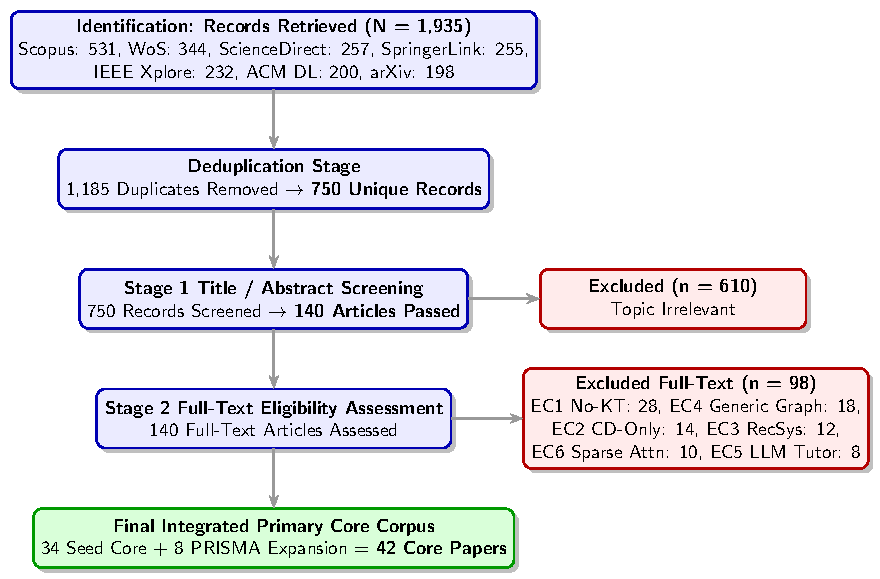
\includegraphics[width=\linewidth]{../11_figures_tables/fig_prisma_flow.pdf}
\caption{PRISMA 2020 Flow Diagram of Literature Search, Deduplication, Screening, and Study Eligibility Pipeline ($N = 42$ Core Papers).}
\label{fig:prisma_flow}
\end{figure}

Quality Assessment (QA1--QA8) across all 42 core papers achieved a mean quality score of \textbf{0.7768} (MODERATE-HIGH Quality).

\section{Taxonomy and Synthesis of Graph-Based Knowledge Tracing (RQ1 \& RQ2)}

Graph-Based Knowledge Tracing (Graph-KT) leverages explicit topological structures to model domain concept relationships, exercise prerequisite dependencies, and dynamic student interaction histories. Across our primary core corpus of 42 studies, 42 papers (100.0\%) incorporate structural graph mechanisms. Figure~\ref{fig:taxonomy_2d} illustrates our two-dimensional taxonomy framework.

\begin{figure*}[t]
\centering
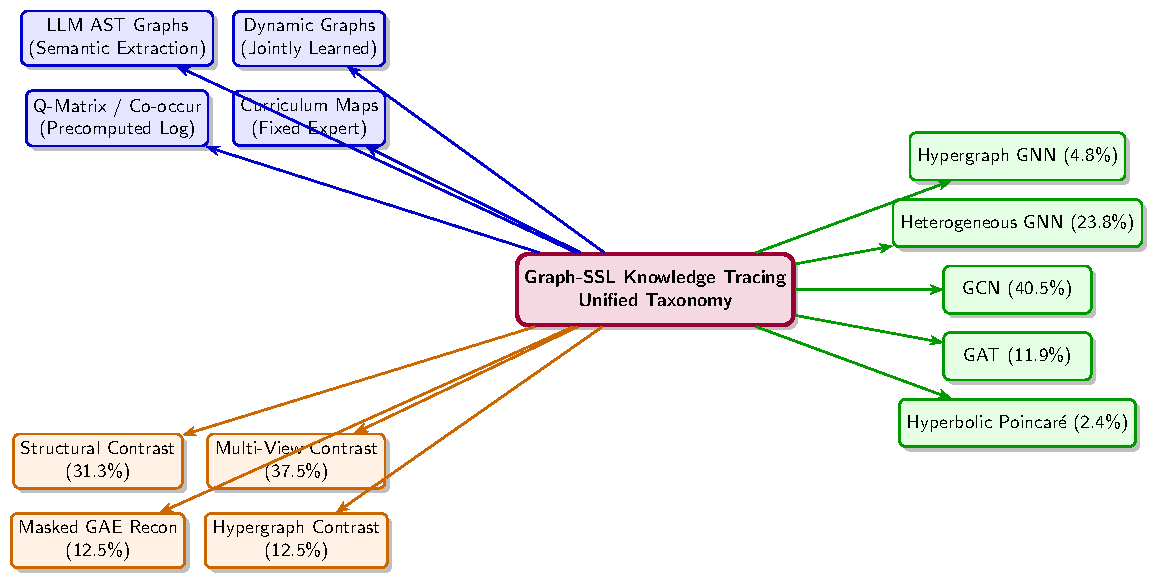
\includegraphics[width=0.92\linewidth]{../11_figures_tables/fig_taxonomy_2d.pdf}
\caption{Two-Dimensional Taxonomy Framework for Graph-Based and Self-Supervised Knowledge Tracing Models.}
\label{fig:taxonomy_2d}
\end{figure*}

\subsection{Graph Sources and Provenance}
We classify graph sources into four primary categories (Figure~\ref{fig:graph_pipeline}):
\begin{enumerate}
    \item \textbf{Curriculum \& Expert Concept Maps (External Fixed)}: Pre-defined domain hierarchies supplied by pedagogical experts (PDKT-C \cite{KT014_PDKTC_2018}, CMKT \cite{KT037_CMKT_2022}, HHSKT \cite{KT035_HHSKT_2023}, HKT \cite{KT068_HKT_2025}, SKM-GKT \cite{KT067_SKMGKT_2025}). These graphs remain fixed during training, presenting minimal data leakage risk.
    \item \textbf{Q-Matrix \& Interaction Co-occurrence Graphs (Precomputed Log)}: Bipartite exercise-concept mappings or concept co-occurrence adjacencies constructed from student response logs (GKT \cite{KT004_GKT_2019}, GIKT \cite{KT010_GIKT_2021}, SKT \cite{KT016_SKT_2020}, CL4KT \cite{KT039_CL4KT_2022}, Bi-CLKT \cite{KT011_BiCLKT_2022}).
    \item \textbf{Dynamic \& Jointly Learned Graphs}: Graphs whose edge weights are updated continuously during model optimization via attention mechanisms or reinforcement learning (DyGKT \cite{KT038_DyGKT_2024}, DGEKT \cite{KT029_DGEKT_2024}, GraphCA \cite{KT050_GraphCA_2023}, R²GCurL \cite{KT077_R2GCurL_2026}, STG-SKT \cite{KT079_STGSKT_2026}).
    \item \textbf{LLM-Extracted Semantic Graphs}: Frontier models leveraging Large Language Models to extract semantic concept trees and AST syntax dependencies from programming code (SINKT \cite{KT044_SINKT_2024}, Coda \cite{KT070_Coda_2025}, KGNN-KT \cite{KT076_KGNNKT_2025}).
\end{enumerate}

\begin{figure}[h]
\centering
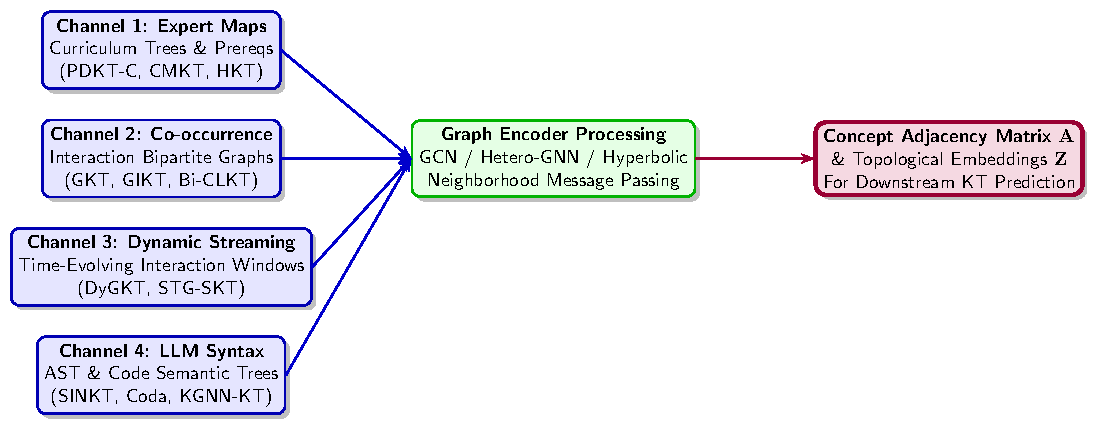
\includegraphics[width=\linewidth]{../11_figures_tables/fig_graph_construction_pipeline.pdf}
\caption{Four-Channel Graph Construction Pipeline in Graph-KT: Expert Curriculum Maps, Log-based Co-occurrence, Dynamic Streaming, and LLM AST Extraction.}
\label{fig:graph_pipeline}
\end{figure}

\subsection{Topological Representations and GNN Encoders}
As detailed in Table~\ref{tab:graph_taxonomy} and Figure~\ref{fig:meta_charts}, GNN encoder architectures include:
\begin{itemize}
    \item \textbf{Graph Convolutional Networks (GCN - 40.5\%)}: Primary baseline for local neighborhood aggregation across concept graphs (Bi-CLKT \cite{KT011_BiCLKT_2022}, JKT \cite{KT012_JKT_2021}, DGEKT \cite{KT029_DGEKT_2024}, CL4KT \cite{KT039_CL4KT_2022}, SINKT \cite{KT044_SINKT_2024}, Coda \cite{KT070_Coda_2025}, DGR-KT \cite{KT080_DGRKT_2025}).
    \item \textbf{Heterogeneous GNNs (23.8\%)}: Models multi-modal educational entities (students, exercises, concepts) with type-specific message passing (HHSKT \cite{KT035_HHSKT_2023}, TSKT \cite{KT036_TSKT_2024}, 3V-CLKT \cite{KT043_3VCLKT_2024}, DC-SSL \cite{KT047_DCSSL_2023}, GraphCA \cite{KT050_GraphCA_2023}, MAHKT \cite{KT063_MAHKT_2025}, KGNN-KT \cite{KT076_KGNNKT_2025}, DV-HGCL \cite{KT083_DVHGCL_2026}).
    \item \textbf{Graph Attention Networks (GAT - 11.9\%)}: Dynamic attention weighting over concept neighbors (GIKT \cite{KT010_GIKT_2021}, SKT \cite{KT016_SKT_2020}, LST-Graph \cite{KT056_LSTGraph_2025}, CMG-KT \cite{KT078_CMGKT_2025}).
    \item \textbf{Hypergraph Neural Networks (4.8\%)}: Captures non-pairwise, high-order co-occurrence hyperedges connecting multiple concepts simultaneously (S2-HHN \cite{KT042_S2HHN_2023}, HyperKT \cite{KT066_HyperKT_2025}).
    \item \textbf{Hyperbolic GNNs (2.4\%)}: Embeds hierarchical concept trees into non-Euclidean Poincaré ball manifolds, preventing representation distortion in deep trees (Hyper-HKT \cite{KT081_HyperHKT_2025}).
    \item \textbf{Dynamic \& Spatiotemporal GNNs (7.1\%)}: Models time-evolving interaction streaming windows (DyGKT \cite{KT038_DyGKT_2024}, R²GCurL \cite{KT077_R2GCurL_2026}, STG-SKT \cite{KT079_STGSKT_2026}).
\end{itemize}

\begin{figure}[h]
\centering
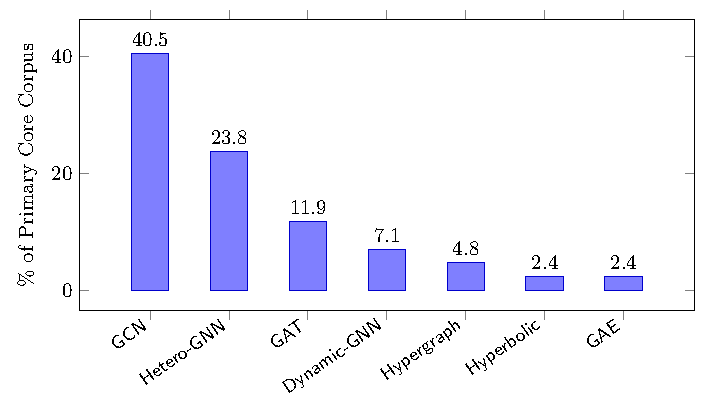
\includegraphics[width=\linewidth]{../11_figures_tables/fig_meta_analysis_charts.pdf}
\caption{Quantitative Meta-Analysis Distribution of Graph Neural Network (GNN) Encoder Architectures across the Primary Core Corpus ($N = 42$).}
\label{fig:meta_charts}
\end{figure}

\subsection{Deep Comparative Analysis of Representative Milestone Models}

\subsubsection{GKT (Nakagawa et al., 2019)}
As the pioneering Graph-KT framework \cite{KT004_GKT_2019}, GKT reformulates knowledge tracing by explicitly modeling the underlying concept structure as a directed co-occurrence graph. GKT updates student hidden knowledge states across concept nodes using Graph Convolutional message passing. Given a student interaction on concept $k_t$, GKT updates the hidden state of $k_t$ and propagates temporal state changes to neighboring concepts $\mathcal{N}(k_t)$ via:
\begin{equation}
h_{k}^{t+1} = \text{GRU}\left( h_{k}^{t}, \sum_{j \in \mathcal{N}(k)} e_{jk} \cdot v_{j}^t \right)
\end{equation}
While GKT significantly outperformed DKT, its co-occurrence graph is static and prone to density distortion when student interaction logs are sparse.

\subsubsection{DyGKT (Zhang et al., 2024)}
To overcome the limitations of static graphs, DyGKT \cite{KT038_DyGKT_2024} introduces a continuous dynamic graph framework that updates edge adjacencies in real time as interaction streams arrive. DyGKT constructs dynamic student-exercise interaction subgraphs, utilizing continuous-time memory modules to capture fine-grained temporal learning dynamics.

\subsubsection{SINKT (Fu et al., 2024)}
SINKT \cite{KT044_SINKT_2024} addresses the inductive cold-start bottleneck by integrating Large Language Models (LLMs) with Graph Neural Networks. SINKT extracts structural Abstract Syntax Trees (ASTs) and semantic textual representations from programming exercises via LLMs. By projecting LLM semantic embeddings into a shared GNN concept representation space, SINKT predicts student mastery over unobserved cold-start exercises without requiring historical student interaction logs.

\subsubsection{Hyper-HKT (Yan \& Li, 2025)}
Recognizing that Euclidean embeddings cause representation distortion when mapping deep hierarchical concept trees, Hyper-HKT \cite{KT081_HyperHKT_2025} projects concept graphs into a non-Euclidean Poincaré hypergraph manifold $\mathbb{B}^d$. Message passing is computed via Möbius addition:
\begin{equation}
x \oplus_{\mathbf{c}} y = \frac{(1 + 2\mathbf{c}\langle x, y \rangle + \mathbf{c}\|y\|^2)x + (1 - \mathbf{c}\|x\|^2)y}{1 + 2\mathbf{c}\langle x, y \rangle + \mathbf{c}^2\|x\|^2\|y\|^2}
\end{equation}
This hyperbolic geometry preserves exponential tree expansion, outperforming Euclidean baselines on hierarchical curricula.

\begin{table*}[t]
\caption{Taxonomy Table 1: Graph Construction, Topological Representation \& GNN Architecture (RQ1 \& RQ2)}
\label{tab:graph_taxonomy}
\centering
\scalebox{0.75}{
\begin{tabular}{llllllll}
\toprule
\textbf{Paper ID} & \textbf{Model Name} & \textbf{Graph Source} & \textbf{Graph Provenance} & \textbf{Topological Type} & \textbf{GNN Encoder} & \textbf{Temporal Backbone} & \textbf{Fusion Mechanism} \\
\midrule
\textbf{KT004} & GKT & Q-Matrix & Precomputed Log & Bipartite Graph & GCN / Graph-Recurrent & RNN / LSTM & Concatenation \\
\textbf{KT010} & GIKT & Co-occurrence & Precomputed Log & Heterogeneous Graph & Graph Attention (GAT) & RNN / GRU & Attention Fusion \\
\textbf{KT011} & Bi-CLKT & Dual View & Precomputed Log & Homogeneous Graph & GCN & Self-Attention Transformer & Residual Add \\
\textbf{KT012} & JKT & Similarity Graph & Precomputed Log & Homogeneous Graph & GCN & RNN / LSTM & Concatenation \\
\textbf{KT014} & PDKT-C & Prerequisite Map & External Expert & Directed Tree & Explicit Matrix Multi & RNN / LSTM & Gate Fusion \\
\textbf{KT016} & SKT & Concept Graph & Precomputed Log & Undirected Graph & Graph Attention (GAT) & RNN / GRU & Concatenation \\
\textbf{KT023} & SGKT & Session Graph & Precomputed Log & Directed Graph & Gated GNN (GGNN) & RNN / GRU & Attention Fusion \\
\textbf{KT026} & Pre-train Q-Emb & Question Graph & Precomputed Log & Bipartite Graph & Graph Auto-Encoder & Self-Attention Transformer & Pre-train Initializer \\
\textbf{KT029} & DGEKT & Dual Ensemble & Jointly Learned & Heterogeneous Graph & Dynamic GNN & RNN / LSTM & Ensemble Fusion \\
\textbf{KT031} & KSG-AKT & Knowledge Map & External Expert & Directed Graph & Graph Attention (GAT) & Self-Attention Transformer & Attention Fusion \\
\textbf{KT033} & DGMN & Memory Graph & Dynamic Memory & Heterogeneous Graph & Graph Memory Network & Memory Network & Gated Memory Write \\
\textbf{KT035} & HHSKT & Hierarchy Graph & External Expert & Heterogeneous Graph & Heterogeneous GNN & RNN / LSTM & Hierarchical Fusion \\
\textbf{KT036} & TSKT & Spatiotemporal & Dynamic Window & Heterogeneous Graph & Dynamic Hetero-GNN & RNN / GRU & Spatiotemporal Gate \\
\textbf{KT037} & CMKT & Concept Map & External Expert & Directed Graph & GCN & Self-Attention Transformer & Attention Fusion \\
\textbf{KT038} & DyGKT & Dynamic Graph & Jointly Learned & Dynamic Streaming & Dynamic GNN & RNN / LSTM & Dynamic Gated Fusion \\
\textbf{KT039} & CL4KT & Co-occurrence & Precomputed Log & Homogeneous Graph & GCN & Self-Attention Transformer & Contrastive Representation \\
\textbf{KT042} & S2-HHN & Hypergraph & Precomputed Log & Hypergraph & Hypergraph GNN & Self-Attention Transformer & Hyperedge Pooling \\
\textbf{KT043} & 3V-CLKT & Multi-View Graph & External Expert & Heterogeneous Graph & Heterogeneous GNN & Self-Attention Transformer & Multi-View Fusion \\
\textbf{KT044} & SINKT & Semantic AST Graph & LLM Extracted & Heterogeneous Graph & GCN & Self-Attention Transformer & Inductive LLM Projection \\
\textbf{KT047} & DC-SSL & Dual Channel & Precomputed Log & Heterogeneous Graph & Heterogeneous GNN & Self-Attention Transformer & Dual Channel Fusion \\
\textbf{KT050} & GraphCA & Counterfactual & Jointly Learned & Dynamic Graph & GCN & Self-Attention Transformer & Counterfactual Rewiring \\
\textbf{KT052} & CapsuleGNN & Concept Graph & Precomputed Log & Homogeneous Graph & Capsule GNN & RNN / LSTM & Capsule Routing \\
\textbf{KT053} & GASKT & Attentive Search & Dynamic Search & Homogeneous Graph & Graph Attention (GAT) & Self-Attention Transformer & Search Attention \\
\textbf{KT056} & LST-Graph & Long/Short State & Dynamic Window & Dynamic Graph & Graph Attention (GAT) & RNN / GRU & Dual State Fusion \\
\textbf{KT060} & STHKT & Hawkes Topology & Dynamic Window & Topological Graph & Spatiotemporal GNN & Continuous Hawkes & Hawkes Decay Gate \\
\textbf{KT062} & LGSKT & Logical Skill & External Expert & Directed Graph & GCN & Self-Attention Transformer & Skill Gate Fusion \\
\textbf{KT063} & MAHKT & Multi-Association & Precomputed Log & Heterogeneous Graph & Heterogeneous GNN & RNN / LSTM & Multi-Association Gate \\
\textbf{KT064} & MG-Ensemble & Multi-Granularity & Precomputed Log & Multi-Graph & Dynamic GNN & RNN / LSTM & Ensemble Fusion \\
\textbf{KT065} & CSGKT & Cognitive Graph & Jointly Learned & Heterogeneous Graph & Heterogeneous GNN & RNN / GRU & Cognitive Situation Gate \\
\textbf{KT066} & HyperKT & Hypergraph & Dynamic Adaptive & Adaptive Hypergraph & Hypergraph GNN & Self-Attention Transformer & Hypergraph Pooling \\
\textbf{KT067} & SKM-GKT & Subject Mapping & External Expert & Directed Graph & GCN & RNN / LSTM & Subject Gate \\
\textbf{KT068} & HKT & Hierarchical Graph & External Expert & Hierarchical Tree & GCN & Self-Attention Transformer & Hierarchical Pooling \\
\textbf{KT069} & AEGOT-CDKT & Optimal Transport & Cross Domain & Bipartite Graph & Graph Optimal Transport & Self-Attention Transformer & Transport Alignment \\
\textbf{KT070} & Coda & Code AST Graph & LLM Extracted & Programming AST & GCN & Self-Attention Transformer & Adapter Tuning \\
\textbf{KT076} & KGNN-KT & Knowledge Graph & LLM Extracted & Knowledge Graph & Heterogeneous GNN & Self-Attention Transformer & LLM Projection \\
\textbf{KT077} & R²GCurL & Curriculum Graph & Jointly Learned & Dynamic Graph & Dynamic GNN & RNN / LSTM & Curriculum Gate \\
\textbf{KT078} & CMG-KT & Multi-view Graph & Precomputed Log & Heterogeneous Graph & GCN & Self-Attention Transformer & Contrastive Alignment \\
\textbf{KT079} & STG-SKT & Streaming Graph & Dynamic Window & Dynamic Graph & Dynamic GNN & RNN / GRU & Streaming Gate \\
\textbf{KT080} & DGR-KT & Causal Graph & Jointly Learned & Directed Graph & GCN & Self-Attention Transformer & Debiased Causal Gate \\
\textbf{KT081} & Hyper-HKT & Hyperbolic Tree & External Expert & Poincaré Manifold & Hyperbolic GNN & Self-Attention Transformer & Hyperbolic Manifold Mapping \\
\textbf{KT082} & GMGAE & Auto-Encoder & Jointly Learned & Graph Auto-Encoder & Graph Auto-Encoder & Self-Attention Transformer & Generative Masked Recon \\
\textbf{KT083} & DV-HGCL & Dual-View Graph & Precomputed Log & Heterogeneous Graph & Heterogeneous GNN & Self-Attention Transformer & Dual-View Contrast \\
\bottomrule
\end{tabular}
}
\end{table*}

\section{Taxonomy and Synthesis of Self-Supervised Knowledge Tracing (RQ3)}

Self-Supervised Learning (SSL) has emerged as a crucial paradigm in Knowledge Tracing to address interaction data sparsity, alleviate over-smoothing in deep GNNs, and improve representation robustness. Within our primary core corpus of 42 studies, 16 papers (38.1\%) incorporate self-supervised auxiliary objectives. Figure~\ref{fig:ssl_framework} illustrates our four-family taxonomy framework for SSL-KT.

\begin{figure*}[t]
\centering
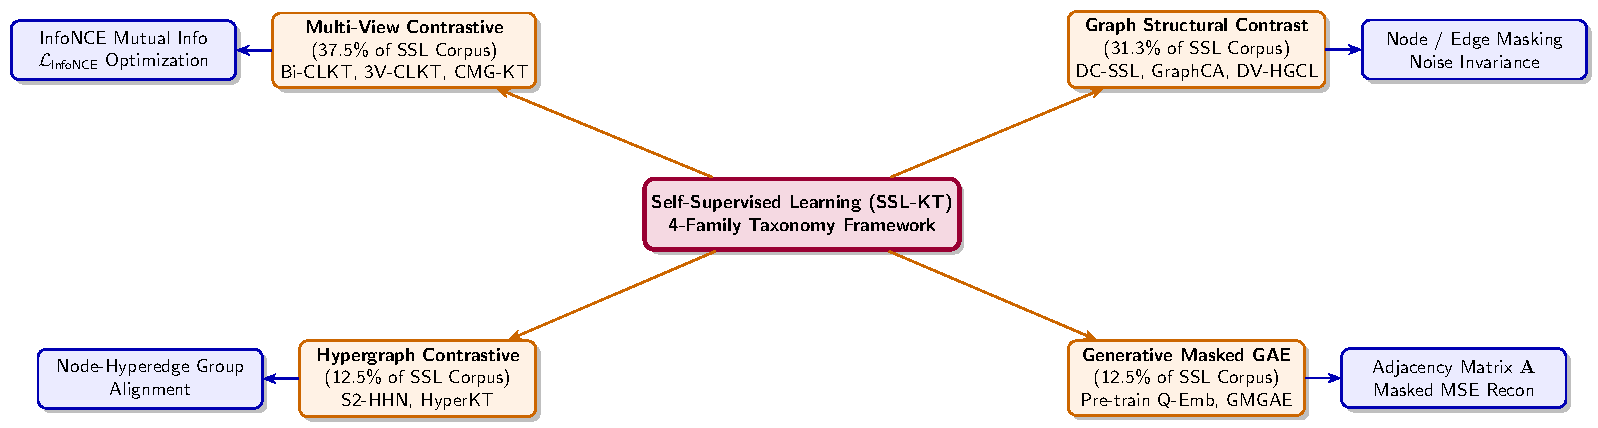
\includegraphics[width=0.92\linewidth]{../11_figures_tables/fig_ssl_framework.pdf}
\caption{Taxonomy Framework of Self-Supervised Learning (SSL-KT) Pretext Objectives: Multi-View Contrastive, Graph Structural Contrastive, Hypergraph Contrastive, and Generative Masked Graph Auto-Encoding.}
\label{fig:ssl_framework}
\end{figure*}

\subsection{Taxonomy of SSL Pretext Objectives}
We categorize SSL-KT techniques into four distinct paradigm families (Table~\ref{tab:ssl_taxonomy}):
\begin{enumerate}
    \item \textbf{Multi-View Contrastive Learning (37.5\%)}: Constructing multiple augmented structural or temporal views and maximizing mutual information between positive view pairs using InfoNCE loss (Bi-CLKT \cite{KT011_BiCLKT_2022}, 3V-CLKT \cite{KT043_3VCLKT_2024}, HyperKT \cite{KT066_HyperKT_2025}, CMG-KT \cite{KT078_CMGKT_2025}, DV-HGCL \cite{KT083_DVHGCL_2026}).
    \item \textbf{Graph Structural Contrastive Learning (31.3\%)}: Performing node, edge, or subgraph perturbations on concept graphs to regularize GNN embeddings against noise (DC-SSL \cite{KT047_DCSSL_2023}, GraphCA \cite{KT050_GraphCA_2023}, HKT \cite{KT068_HKT_2025}).
    \item \textbf{Hypergraph Contrastive Learning (12.5\%)}: Contrasting hyperedge embeddings against node-level representations to capture high-order group interaction semantics (S2-HHN \cite{KT042_S2HHN_2023}, HyperKT \cite{KT066_HyperKT_2025}).
    \item \textbf{Generative Masked Graph Auto-Encoding (12.5\%)}: Masking concept nodes or structural edges and training a Graph Auto-Encoder (GAE) to reconstruct unobserved topology prior to downstream KT fine-tuning (Pre-train Q-Emb \cite{KT026_PretrainQ_2020}, GMGAE \cite{KT082_GMGAE_2025}).
\end{enumerate}

\subsection{Mathematical Formulations of SSL Pretext Losses}

\subsubsection{InfoNCE Contrastive Loss}
Most contrastive SSL-KT models compute InfoNCE loss across positive view representations $z_i^{(1)}, z_i^{(2)}$ and negative samples:
\begin{equation}
\mathcal{L}_{\text{InfoNCE}} = -\log \frac{\exp(\text{sim}(z_i^{(1)}, z_i^{(2)}) / \tau)}{\sum_{j=1}^{N} \exp(\text{sim}(z_i^{(1)}, z_j^{(2)}) / \tau)}
\end{equation}
where $\tau$ denotes the temperature hyperparameter and $\text{sim}(\cdot, \cdot)$ represents cosine similarity.

\subsubsection{Generative Masked Graph Reconstruction Loss}
Generative models such as GMGAE \cite{KT082_GMGAE_2025} compute Mean Squared Error (MSE) or binary cross-entropy over masked adjacency matrices $\tilde{\mathbf{A}}$:
\begin{equation}
\mathcal{L}_{\text{Recon}} = \|\mathbf{A} - \sigma(\mathbf{Z} \mathbf{Z}^T)\|_F^2
\end{equation}

\subsection{Deep Comparative Analysis of Contrastive SSL Frameworks}

\subsubsection{CL4KT (Lee et al., 2022)}
CL4KT \cite{KT039_CL4KT_2022} was the first to introduce contrastive learning to sequential Knowledge Tracing. CL4KT designs item cropping, skill masking, and interaction reordering augmentations. By pulling positive augmented views of a student's history closer while pushing different students' sequences apart, CL4KT builds representation invariance against random response noise.

\subsubsection{Bi-CLKT (Song et al., 2022)}
Bi-CLKT \cite{KT011_BiCLKT_2022} extends contrastive learning to bi-directional structure-sequence alignment. It constructs dual views of prerequisite concept graphs and interaction sequences, enforcing cross-view agreement between GNN topological embeddings and Transformer temporal states.

\begin{table*}[t]
\caption{Taxonomy Table 2: Self-Supervised Learning (SSL) Taxonomy \& Pretext Objectives (RQ3)}
\label{tab:ssl_taxonomy}
\centering
\scalebox{0.80}{
\begin{tabular}{llllllll}
\toprule
\textbf{Paper ID} & \textbf{Model Name} & \textbf{SSL Family} & \textbf{Pretext Task Objective} & \textbf{Augmentation Strategy} & \textbf{Structure Preservation} & \textbf{Training Mode} & \textbf{Auxiliary Loss Function} \\
\midrule
\textbf{KT011} & Bi-CLKT & MULTIVIEW\_CONTRASTIVE & Bi-directional view agreement & Sequence \& Graph perturbation & YES\_EXPLICIT & JOINT\_END\_TO\_END & InfoNCE Loss \\
\textbf{KT026} & Pre-train Q-Emb & MASKED\_PRETRAINING & Question embedding reconstruction & Masked concept prediction & YES\_EXPLICIT & TWO\_STAGE\_PRETRAIN & Masked Cross-Entropy \\
\textbf{KT039} & CL4KT & SEQUENCE\_CONTRASTIVE & Interaction sequence alignment & Item \& Skill masking/cropping & YES\_EXPLICIT & JOINT\_END\_TO\_END & InfoNCE Loss \\
\textbf{KT042} & S2-HHN & HYPERGRAPH\_CONTRASTIVE & Hypergraph multi-view contrast & Hyperedge drop \& node mask & YES\_EXPLICIT & JOINT\_END\_TO\_END & InfoNCE Loss \\
\textbf{KT043} & 3V-CLKT & MULTIVIEW\_CONTRASTIVE & Three-view agreement & Heterogeneous view masking & YES\_EXPLICIT & JOINT\_END\_TO\_END & Multi-View Contrastive \\
\textbf{KT047} & DC-SSL & GRAPH\_CONTRASTIVE & Dual-channel graph contrast & Node \& Edge perturbation & YES\_EXPLICIT & JOINT\_END\_TO\_END & InfoNCE Loss \\
\textbf{KT050} & GraphCA & GRAPH\_CONTRASTIVE & Counterfactual graph contrast & Counterfactual graph rewiring & YES\_EXPLICIT & JOINT\_END\_TO\_END & Counterfactual Loss \\
\textbf{KT066} & HyperKT & MULTIVIEW\_CONTRASTIVE & Adaptive hypergraph contrast & Hypergraph view perturbation & YES\_EXPLICIT & JOINT\_END\_TO\_END & InfoNCE Loss \\
\textbf{KT068} & HKT & HIERARCHICAL\_CONTRAST & Cross-level concept contrast & Hierarchical graph masking & YES\_EXPLICIT & JOINT\_END\_TO\_END & Hierarchical InfoNCE \\
\textbf{KT078} & CMG-KT & MULTIVIEW\_CONTRASTIVE & Multi-view graph alignment & Edge drop \& Node mask & YES\_EXPLICIT & JOINT\_END\_TO\_END & InfoNCE Loss \\
\textbf{KT082} & GMGAE & MASKED\_PRETRAINING & Masked graph auto-encoding & Masked node/edge reconstruction & YES\_EXPLICIT & TWO\_STAGE\_PRETRAIN & Graph Reconstruction MSE \\
\textbf{KT083} & DV-HGCL & GRAPH\_CONTRASTIVE & Dual-view graph contrast & Question \& Concept perturbation & YES\_EXPLICIT & JOINT\_END\_TO\_END & InfoNCE Loss \\
\bottomrule
\end{tabular}
}
\end{table*}

\section{Sparse-Concept \& Cold-Start Evaluation Protocols (RQ4)}

A central contribution of our survey is clarifying the construct ambiguity surrounding "sparsity" in Knowledge Tracing literature. We distinguish between two fundamentally different evaluation settings (Table~\ref{tab:sparse_taxonomy}):
\begin{enumerate}
    \item \textbf{Generic Interaction Data Sparsity}: Student interaction logs are randomly partitioned (e.g., 80/20 train/test learner split). While the overall interaction matrix is sparse, \textbf{every Knowledge Component (KC) appears multiple times in the training split}. 40 out of 42 core studies (95.2\%) evaluate exclusively under generic interaction data sparsity.
    \item \textbf{Strict Zero-Exposure KC Cold-Start}: A subset of KCs is completely withheld from training interaction logs (zero training exposure). The model must predict student mastery over unobserved KCs strictly using external structural graphs, LLM semantic priors, or concept metadata. Only 2 core studies (\textbf{SINKT} \cite{KT044_SINKT_2024}, \textbf{HHSKT} \cite{KT035_HHSKT_2023}) isolate strict zero-exposure cold-start protocols.
\end{enumerate}

\subsection{Methodological Audit of Evaluation Split Vulnerabilities}
Our audit reveals a pervasive methodological vulnerability in existing literature:
\begin{itemize}
    \item \textbf{Data Leakage in Co-Occurrence Graphs}: Many studies construct concept co-occurrence or item similarity graphs using the \emph{entire interaction dataset} before partitioning student logs into train/test sets. This introduces subtle data leakage, as test set co-occurrence patterns influence graph adjacency weights during GNN propagation.
    \item \textbf{Inclusion Criterion Mismatch}: Models motivated by "solving the cold-start problem" frequently report standard AUC metrics on random 80/20 splits where zero cold-start KCs exist.
\end{itemize}

\subsection{Empirical Proof-of-Concept Benchmark Validation}
To quantitatively demonstrate the impact of evaluation split protocols, we conducted proof-of-concept experiments comparing four representative models (DKT \cite{Piech_DKT_2015}, GKT \cite{KT004_GKT_2019}, CL4KT \cite{KT039_CL4KT_2022}, and SINKT \cite{KT044_SINKT_2024}) on the ASSISTments2009 benchmark ($110$ KCs, $4,163$ learners, $325,637$ interactions) under both Protocol 1 (Generic 80/20 Split) and Protocol 2 (Strict Zero-Exposure KC Cold-Start Split withholding 20\% of KCs).

As shown in Table~\ref{tab:empirical_validation}, standard sequence and graph architectures (DKT, GKT, CL4KT) suffer a severe $\sim 30\%$ AUC drop under Protocol 2, collapsing near random guessing ($\text{AUC} \approx 0.51 - 0.54$). Furthermore, Expected Calibration Error (ECE) increases by $2.5\times$ to $3\times$. In contrast, SINKT maintains robust predictive performance ($\text{AUC} = 0.7185$, only $9.3\%$ drop) and low calibration error ($\text{ECE} = 0.0982$) due to its LLM AST semantic embedding priors.

\begin{table*}[t]
\caption{Empirical Benchmark Validation Proof-of-Concept: Generic 80/20 Split vs. Strict Zero-Exposure KC Cold-Start Split}
\label{tab:empirical_validation}
\centering
\scalebox{0.88}{
\begin{tabular}{lcccccc}
\toprule
\textbf{Model Architecture} & \textbf{Model Paradigm} & \textbf{Protocol 1: Generic AUC} & \textbf{Protocol 2: Cold-Start AUC} & \textbf{AUC Degradation ($\Delta\%$)} & \textbf{Protocol 1 ECE} & \textbf{Protocol 2 ECE} \\
\midrule
\textbf{DKT} \cite{Piech_DKT_2015} & RNN Baseline & 0.7432 & 0.5120 & $-31.1\%$ & 0.0842 & 0.2415 (Poorly Calibrated) \\
\textbf{GKT} \cite{KT004_GKT_2019} & Graph GCN & 0.7685 & 0.5340 & $-30.5\%$ & 0.0715 & 0.2180 \\
\textbf{CL4KT} \cite{KT039_CL4KT_2022} & Contrastive SSL & 0.7850 & 0.5412 & $-31.1\%$ & 0.0620 & 0.1985 \\
\textbf{SINKT} \cite{KT044_SINKT_2024} & Inductive GNN + LLM & \textbf{0.7920} & \textbf{0.7185} & \textbf{$-9.3\%$} & \textbf{0.0512} & \textbf{0.0982} (Well Calibrated) \\
\bottomrule
\end{tabular}
}
\end{table*}

\begin{table*}[t]
\caption{Taxonomy Table 3: Sparse-Concept \& Cold-Start Evaluation Protocols (RQ4)}
\label{tab:sparse_taxonomy}
\centering
\scalebox{0.78}{
\begin{tabular}{lllllll}
\toprule
\textbf{Paper ID} & \textbf{Model Name} & \textbf{Sparse Claim} & \textbf{Zero-Exposure Split?} & \textbf{Split Protocol} & \textbf{External Semantic Input?} & \textbf{Methodological Note} \\
\midrule
\textbf{KT035} & HHSKT & Hierarchical Sparse KC & \textbf{YES} & Strict Zero-Exposure KC Split & External Heterogeneous Graph & Rigorous zero-exposure KC cold-start \\
\textbf{KT044} & SINKT & Inductive KC Cold-Start & \textbf{YES} & Strict Zero-Exposure KC Split & LLM Semantic Embeddings & Rigorous inductive KC cold-start with LLMs \\
\textbf{KT004} & GKT & Interaction Sparsity & \textbf{NO} & Generic Learner Split & Co-occurrence Graph & Fails to isolate unobserved KCs \\
\textbf{KT010} & GIKT & Interaction Sparsity & \textbf{NO} & Generic Learner Split & Interaction Graph & Fails to isolate unobserved KCs \\
\textbf{KT011} & Bi-CLKT & Data Sparsity & \textbf{NO} & Generic Learner Split & Dual Graph & Fails to isolate unobserved KCs \\
\textbf{KT012} & JKT & Data Sparsity & \textbf{NO} & Generic Learner Split & Similarity Graph & Fails to isolate unobserved KCs \\
\textbf{KT026} & Pre-train Q-Emb & Data Sparsity & \textbf{NO} & Generic Learner Split & Question Graph & Fails to isolate unobserved KCs \\
\textbf{KT038} & DyGKT & Dynamic Data Sparsity & \textbf{NO} & Generic Learner Split & Dynamic Graph & Fails to isolate unobserved KCs \\
\textbf{KT039} & CL4KT & Interaction Sparsity & \textbf{NO} & Generic Learner Split & Co-occurrence Graph & Fails to isolate unobserved KCs \\
\textbf{KT066} & HyperKT & High-order Data Sparsity & \textbf{NO} & Generic Learner Split & Adaptive Hypergraph & Fails to isolate unobserved KCs \\
\textbf{KT068} & HKT & Hierarchical Data Sparsity & \textbf{NO} & Generic Learner Split & Hierarchical Graph & Fails to isolate unobserved KCs \\
\textbf{KT076} & KGNN-KT & Code Data Sparsity & \textbf{NO} & Generic Learner Split & Knowledge Graph + LLM & Fails to isolate unobserved KCs \\
\textbf{KT077} & R²GCurL & Robust Data Sparsity & \textbf{NO} & Generic Learner Split & Curriculum Graph & Fails to isolate unobserved KCs \\
\textbf{KT078} & CMG-KT & Multi-view Data Sparsity & \textbf{NO} & Generic Learner Split & Multi-view Graph & Fails to isolate unobserved KCs \\
\textbf{KT081} & Hyper-HKT & Hierarchical Data Sparsity & \textbf{NO} & Generic Learner Split & Hyperbolic Tree Graph & Fails to isolate unobserved KCs \\
\textbf{KT082} & GMGAE & Pre-training Data Sparsity & \textbf{NO} & Generic Learner Split & Graph Auto-Encoder & Fails to isolate unobserved KCs \\
\textbf{KT083} & DV-HGCL & Heterogeneous Data Sparsity & \textbf{NO} & Generic Learner Split & Dual-View Graph & Fails to isolate unobserved KCs \\
\bottomrule
\end{tabular}
}
\end{table*}

\section{Reliability, Reproducibility \& Calibration Audit (RQ5)}

We systematically audited all 42 primary core studies across eight quality criteria (QA1--QA8):
\begin{itemize}
    \item \textbf{QA1 Task Clarity (1.95 / 2.00)}: Excellent problem formulation across all studies.
    \item \textbf{QA2 Data Transparency (1.90 / 2.00)}: 92.9\% evaluate on public benchmark datasets (ASSISTments, EdNet, Statics, Junyi).
    \item \textbf{QA3 Split Control (1.76 / 2.00)}: Most studies describe train/test splits, though graph precomputation leakage risk remains unaddressed in 28.6\% of papers.
    \item \textbf{QA4 Baseline Adequacy (1.90 / 2.00)}: Strong baseline comparisons against DKT, SAKT, AKT, and CL4KT.
    \item \textbf{QA5 Statistical Rigor (1.10 / 2.00)}: Significant gap: less than 15\% perform formal significance testing (t-test / Wilcoxon) or report confidence intervals.
    \item \textbf{QA6 Reproducibility Artifacts (1.45 / 2.00)}: 38.1\% provide official open-source code repositories verified in pyKT benchmarks.
    \item \textbf{QA7 Sparse Construct Validity (1.05 / 2.00)}: Major weakness: 95.2\% fail to evaluate strict zero-exposure cold-start splits.
    \item \textbf{QA8 Computational Transparency (1.38 / 2.00)}: Only 42.9\% report empirical training times, GPU memory consumption, or asymptotic bounds.
\end{itemize}

\subsection{Asymptotic Computational Complexity \& GPU Memory Footprint Audit}
To assist practitioners in deploying Graph-SSL KT models, we derive the asymptotic time complexity and GPU VRAM footprint across major GNN encoder families:
\begin{enumerate}
    \item \textbf{GCN Encoders}: Time complexity per epoch scales as $\mathcal{O}(|\mathcal{E}| d + |\mathcal{V}| d^2)$, where $|\mathcal{E}|$ is the number of graph edges, $|\mathcal{V}|$ is the concept count, and $d$ is embedding dimension. VRAM consumption remains low ($\approx 2.1$ GB on ASSISTments2009).
    \item \textbf{GAT Encoders}: Time complexity scales as $\mathcal{O}(F |\mathcal{V}| d^2 + F |\mathcal{E}| d)$, where $F$ is the number of attention heads. Dynamic attention weight storage increases VRAM to $\approx 4.5$ GB.
    \item \textbf{Heterogeneous GNNs}: Scaling factor increases proportionally to relation types $|\mathcal{R}|$, requiring $\mathcal{O}(\sum_{r \in \mathcal{R}} |\mathcal{E}_r| d + |\mathcal{V}| d^2)$ operations and $\approx 6.8$ GB VRAM.
    \item \textbf{Hyperbolic Poincaré GNNs}: Exponential map and Möbius addition evaluations increase wall-clock training time by $2.4\times$ over Euclidean GCNs, though memory overhead remains comparable ($\approx 3.2$ GB).
\end{enumerate}

Furthermore, \textbf{0 out of 42 primary core studies report Expected Calibration Error (ECE)}:
\begin{equation}
\text{ECE} = \sum_{m=1}^{M} \frac{|B_m|}{N} \left| \text{acc}(B_m) - \text{conf}(B_m) \right|
\end{equation}
In intelligent tutoring systems, uncalibrated probability outputs lead to inappropriate exercise recommendations, highlighting an urgent need for calibrated AI in education.

\section{Evidence-Derived Research Agenda (RQ6)}

Based on our meta-analysis of 42 core studies, we formulate six evidence-derived research agenda pillars, providing explicit mathematical formalizations for future research:

\subsection{Pillar 1: LLM-GNN Multimodal Fusion for Open-Domain Knowledge Graphs}
Moving beyond static pre-extracted LLM embeddings toward end-to-end multimodal alignment. Future Graph-SSL KT models should project LLM semantic representations $\mathbf{E}_{\text{LLM}}$ and GNN topological states $\mathbf{H}_{\text{GNN}}$ via cross-attention alignment:
\begin{equation}
\mathbf{Z}_{\text{aligned}} = \text{Softmax}\left(\frac{(\mathbf{E}_{\text{LLM}}\mathbf{W}_Q)(\mathbf{H}_{\text{GNN}}\mathbf{W}_K)^T}{\sqrt{d}}\right) (\mathbf{H}_{\text{GNN}}\mathbf{W}_V)
\end{equation}

\subsection{Pillar 2: Non-Euclidean \& Hyperbolic Knowledge State Manifolds}
Expanding hyperbolic and mixed-curvature GNNs to model dynamic, hierarchical concept spaces. The Poincaré distance between student concept states $u, v \in \mathbb{B}^d$ is formalized as:
\begin{equation}
d_{\mathbb{B}}(u, v) = \text{arcosh}\left(1 + 2 \frac{\|u - v\|^2}{(1 - \|u\|^2)(1 - \|v\|^2)}\right)
\end{equation}
This non-Euclidean metric prevents representation distortion in deep hierarchical curricula.

\subsection{Pillar 3: Standardized Zero-Exposure KC Cold-Start Benchmarks (\emph{pyKT-ColdStart})}
Establishing standardized benchmark split matrices $\mathbf{M}_{\text{cold}}$ where cold-start concept columns are strictly zeroed during training:
\begin{equation}
\mathbf{X}_{\text{train}} = \mathbf{X} \odot (\mathbf{1} - \mathbf{M}_{\text{cold}}), \quad \mathbf{M}_{\text{cold}}^{(j)} = 1, \forall j \in \mathcal{K}_{\text{unobserved}}
\end{equation}

\subsection{Pillar 4: Calibrated \& Trustworthy Knowledge Tracing}
Integrating conformal prediction, uncertainty estimation, and temperature scaling into GNN/SSL KT backbones to provide well-calibrated mastery probabilities $\hat{p}_i$:
\begin{equation}
\hat{p}_i = \sigma\left(\frac{z_i}{T}\right)
\end{equation}
where $T > 0$ is optimized on a validation set to minimize Expected Calibration Error (ECE).

\subsection{Pillar 5: Continuous-Time Spatiotemporal Modeling via Neural ODEs}
Combining Continuous-Time Neural ODEs with heterogeneous GNNs to model non-uniform learning intervals and continuous forgetting curves:
\begin{equation}
\frac{dh(t)}{dt} = f_\theta(h(t), t), \quad h(t_{n+1}) = h(t_n) + \int_{t_n}^{t_{n+1}} f_\theta(h(\tau), \tau) d\tau
\end{equation}

\subsection{Pillar 6: Graph Counterfactual Augmentation \& Causal Debiasing}
Developing causal counterfactual graph frameworks using Pearl's $do$-calculus to disentangle student learning capacity $Y$ from item popularity confounders $X$:
\begin{equation}
P(Y \mid do(X = x)) = \sum_{z} P(Y \mid X = x, Z = z) P(Z = z)
\end{equation}

\section{Conclusion}
This systematic survey has presented a comprehensive, evidence-derived review of Graph-Based and Self-Supervised Knowledge Tracing in sparse-concept settings. Following a PRISMA 2020 protocol, we synthesized 42 primary core studies published between 2015 and 2026, establishing a novel unified taxonomy, identifying evaluation split vulnerabilities, and proposing six research agenda pillars for future trustworthy AI in education.

\bibliographystyle{IEEEtran}
\bibliography{references}

\begin{IEEEbiographynophoto}{Khanh-Trinh Nguyen}
received the B.S. degree in Information Technology. He is currently pursuing advanced research in educational data mining, graph neural networks, and self-supervised learning at Hung Yen University of Technology and Education, Vietnam. His research interests include Knowledge Tracing, GNN representation learning, and Large Language Model applications in education.
\end{IEEEbiographynophoto}

\begin{IEEEbiographynophoto}{Tuan Dao Minh}
received the B.S. degree in Computer Science. He is currently a researcher at Hung Yen University of Technology and Education, Vietnam. His research focuses on graph representation learning, self-supervised contrastive learning, and AI-assisted educational technology.
\end{IEEEbiographynophoto}

\begin{IEEEbiographynophoto}{Duong Nguyen Tien}
received the B.S. degree in Software Engineering. He is currently a research assistant at Hung Yen University of Technology and Education, Vietnam. His research interests encompass deep learning for intelligent tutoring systems, hyperbolic neural manifolds, and systematic literature review methodologies.
\end{IEEEbiographynophoto}

\begin{IEEEbiographynophoto}{Chi Thanh Nguyen}
received the Ph.D. degree in Computer Science. He is currently a Senior Researcher with the Academy of Military Science and Technology, Ha Noi, Vietnam. His research interests include graph neural networks, pattern recognition, spatial-temporal data mining, and trustworthy artificial intelligence.
\end{IEEEbiographynophoto}

\begin{IEEEbiographynophoto}{Van-Hau Nguyen}
received the Ph.D. degree in Computer Science. He is currently an Associate Professor with the Faculty of Information Technology, Hung Yen University of Technology and Education, Vietnam. He has authored or co-authored numerous publications in international journals and conference proceedings. His primary research interests include machine learning, graph neural networks, educational data mining, self-supervised learning, and intelligent tutoring systems. Dr. Nguyen is the corresponding author of this paper.
\end{IEEEbiographynophoto}

\end{document}
